\begin{enumerate}[label=\thesubsection.\arabic*,ref=\thesubsection.\theenumi]
\item An arch is in the form of a parabola with its axis vertical. The arch is 10m high and 5m wide at the base. How wide is it 2m from the vertex of the parabola?
\label{chapters/11/11/5/2}
%\iffalse

\documentclass[journal,10pt,twocolumn]{article}
\usepackage{graphicx}
\usepackage[margin=0.5in]{geometry}
\usepackage[cmex10]{amsmath}
\usepackage{array}
\usepackage{booktabs}
\usepackage{mathtools}
\usepackage{amssymb}
\title{\textbf{Conics Assignment}}
\author{lakshmi kamakshi}
\date{September 2022}
\providecommand{\norm}[1]{\left\lVert#1\right\rVert}
\providecommand{\abs}[1]{\left\vert#1\right\vert}
\let\vec\mathbf
\newcommand{\myvec}[1]{\ensuremath{\begin{pmatrix}#1\end{pmatrix}}}
\newcommand{\mydet}[1]{\ensuremath{\begin{vmatrix}#1\end{vmatrix}}}
\providecommand{\brak}[1]{\ensuremath{\left(#1\right)}}

\begin{document}

\maketitle
\paragraph{\textit{Problem Statement} -
\fi
\\
\solution
	\begin{figure}[!ht]
		\centering
 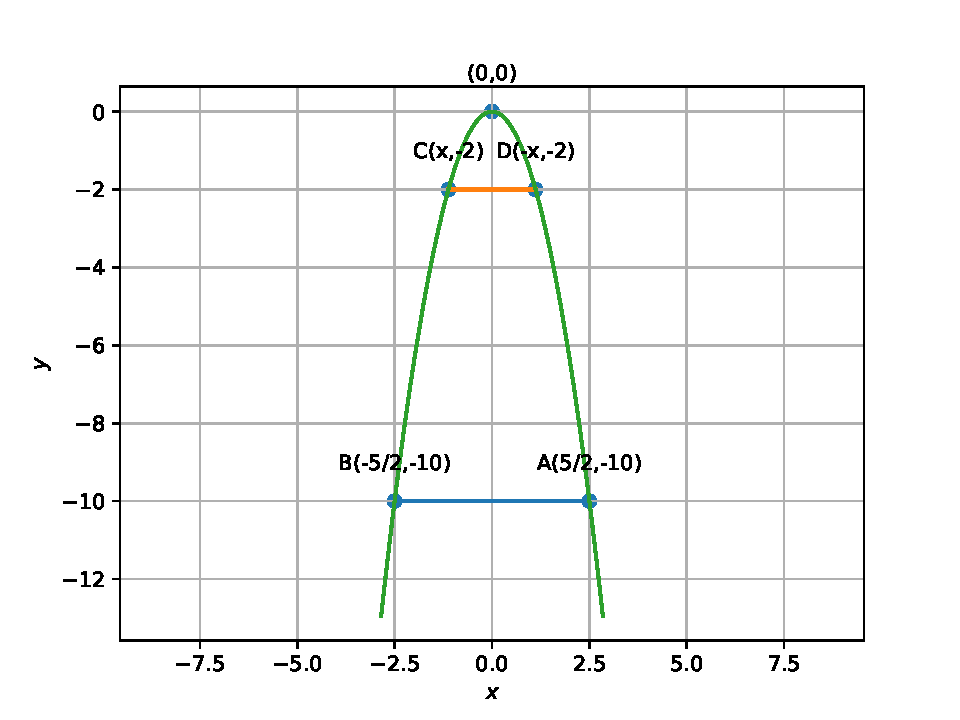
\includegraphics[width=\columnwidth]{chapters/11/11/5/2/figs/fig.pdf}
		\caption{}
		\label{fig:11/11/5/2}
  	\end{figure}
	\iffalse
} \vspace{5mm}

\section*{\large Solution}


Given, the axis of parabola is vertical,
\\ Let the equation of the axis be y-axis:
\begin{equation}
	\label{eq:parabola_q}
	\myvec{1\\0}\textbf{x}= 0
\end{equation}
\\ The above quadratic equation can be written in the general quadratic form as:

\begin{figure}[h]
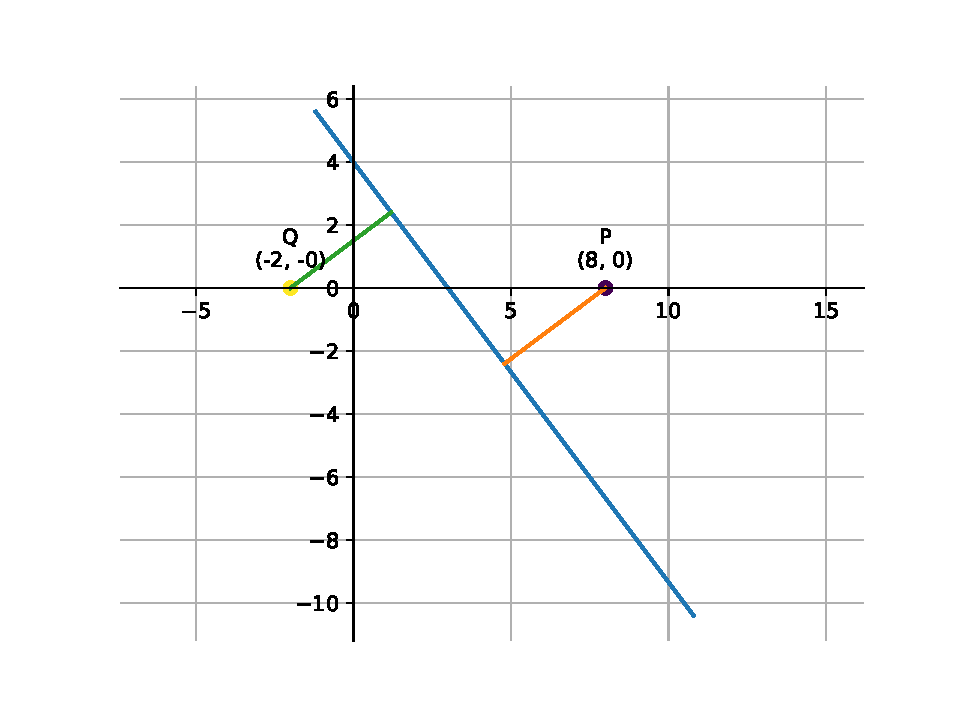
\includegraphics[width=0.8\columnwidth]{fig.pdf}
\end{figure}
\begin{equation}
	\label{eq:std_parabola}
	\textbf{x}^T\textbf{V}\textbf{x}+2\textbf{u}^T\textbf{x}+f=0
\end{equation}
where,
\begin{eqnarray}
\label{eq:Vec_V}
V = \myvec{1&0\\0&0}
\label{eq:Vec_U}
\\ u=\myvec{0\\2a}
\end{eqnarray}
\begin{equation}
\\ f =0
\end{equation}
Given arch is 10m high and 5m wide at the base. So the point $(\frac{5}{2},-10)$ lies on the parabola
\begin{equation}
	\myvec{X_1} = \myvec{\frac{5}{2}\\-10}
\end{equation}
\\ Substitute the point $X_1$ \\
\begin{eqnarray}
	\myvec{X_1}^T \myvec{V} \myvec{X_1} +2\myvec{u^T} \myvec{X_1} = 0
\\	a = \frac{5}{32}
\end{eqnarray}
\\Now , the matrix u will be,
\begin{equation}
	\myvec{u} = \myvec{0\\\frac{5}{16}}
\end{equation}
\\We need to find the width of parabola at a height of $2m$ from the vertex.So,the line parallel to x axis and passing through point $(0,-2)$ intersects the conic at 2 places C and D.
\\The line parallel to x-axis and passing through point $(0,-2)$ is
\begin{align}
	\myvec{X}\myvec{0\\1}^T = \myvec{2}
\end{align}
The points of intersection of the line 
\begin{align}
	L: \quad \vec{x} = \vec{q} + \mu \vec{m} \quad \mu \in \mathbf{R}
\label{eq:conic_tangent}
\end{align}
with the conic section  are given by
\begin{align}
\vec{x}_i = \vec{q} + \mu_i \vec{m}
\label{eq:conic_tangent_pts}
\end{align}
where 
{\tiny
\begin{multline}
\mu_i = \frac{1}
{
\vec{m}^T\vec{V}\vec{m}
}
\lbrak{-\vec{m}^T\brak{\vec{V}\vec{q}+\vec{u}}}
\\
\pm
\rbrak{\sqrt{
\sbrak{
\vec{m}^T\brak{\vec{V}\vec{q}+\vec{u}}
}^2
-
\brak
{
\vec{q}^T\vec{V}\vec{q} + 2\vec{u}^T\vec{q} +f
}
\brak{\vec{m}^T\vec{V}\vec{m}}
	}}
\label{eq:tangent_roots}
\end{multline}
}
\\
Substituting the line in the conic
\begin{align}
\brak{\vec{q} + \mu \vec{m}}^T\vec{V}\brak{\vec{q} + \mu \vec{m}}  
\\
+ 2 \vec{u}^T\brak{\vec{q} + \mu \vec{m}}+f &= 0
\\
\implies \mu^2\vec{m}^T\vec{V}\vec{m} + 2 \mu\vec{m}^T\brak{\vec{V}\vec{q}+\vec{u}} 
\\
+ \vec{q}^T\vec{V}\vec{q} + 2\vec{u}^T\vec{q} +f &= 0
\label{eq:conic_intercept}
\end{align}
Solving the above quadratic equations yeilds the roots.Let the point of intersections of line and curve be C and D.
\begin{align}
	C = q+ \mu_1m
	\\ D = q+ \mu_2m
\end{align}
\\The line CD will be
\begin{align}
	C-D = m(\mu_1-\mu_2)
	 \\ \textbf{m} = \myvec{1\\0}
\end{align}
The required width of parabola is the norm of the line CD.
\begin{align}
	||\boldsymbol{C-D}|| =
	2\sqrt{
\sbrak{
\vec{m}^T\brak{\vec{V}\vec{q}+\vec{u}}
}^2
-
\brak
{
\vec{q}^T\vec{V}\vec{q} + 2\vec{u}^T\vec{q} +f
}}
\end{align}
substitute the values of \vec{m},\vec{q},\vec{V} and \vec{u}
\begin{align}
	\frac{1}{2}||\vec{C-D}||^2 =
	\myvec{1&0}\brak{\vec{V}\myvec{0\\-2}+\vec{u}}\brak{\vec{V}\myvec{0\\-2}+\vec{u}}^T-
\end{align}
\begin{align*}
\brak
{
	\myvec{0&-2}\vec{V}\myvec{0\\-2} + 2\vec{u}^T\myvec{0\\-2} 
}
\end{align*}
 \begin{multiline}
	 \implies \sbrak{\myvec{1&0}\brak{\myvec{1&0\\0&0}\myvec{0\\-2} + \myvec{0\\\frac{5}{16}}}} \brak{\myvec{1&0\\0&0}\myvec{0\\-2} + \myvec{0\\\frac{5}{16}}}}^T  - \\
	 \\ \brak{\myvec{0&-2}\myvec{1&0\\0&0}\myvec{0\\-2} + 2\myvec{0 & \frac{5}{16}}\myvec{0\\-2} - 0} \\ \brak{\myvec{1&0}\myvec{1&0\\0&0}\myvec{1\\0}}
\end{multline}
\begin{align}
	\implies \sbrak{\myvec{1&0}\myvec{0\\\frac{5}{16}}}^2 - \brak{\myvec{0\\0}+2\myvec{0\\\frac{5}{-8}} - 0}(1) \\
 & = \myvec{5\\2}
\end{align}
\\The width of the Parabola at $2m$ height is the length of the line CD.  \begin{align} ||\vec{C-D}|| = \myvec{\sqrt{5}}$m$ \end{align} \section*{\large Construction} The input parameters are V,u,$X_1$,$y_2$ \\
\setlength\extrarowheight{7pt}
\begin{tabular}{|c|c|c|}
	\hline
	\textbf{Symbol}&\textbf{Value}&\textbf{Description}\\
	\hline
	$X_1$=\myvec{x_1\\y_1} & \myvec{\frac{5}{2}\\-10}&point at base \\[8pt]
	\hline
	$y_2$ & -2& height of point C\\[8pt]
	\hline
	$\vec{P}$&\myvec{0&1\\1&0}&eigenvectors of $\vec{V}$\\[8pt]
	\hline
	$\vec{c}$&$\myvec{0\\0}$&center of parabola\\
	\hline
	$\eta$&$\vec{u}^{\top}\vec{p}_1$&from Eq11\\[8pt]
	\hline
	$\lambda_2$&$\vec{e}_2^{\top}D\vec{e}_2$&from Eq9 \\[8pt]
	\hline
	$(\vec{A},\vec{B})$&\myvec{x_1&-x_1\\y_1&y_1}&points at the base\\[8pt]
	\hline
	$(\vec{C},\vec{D})$&\myvec{\sqrt{\frac{5y_2}{8}}&\sqrt{\frac{-5y_2}{8}}\\2&2}&points at 2m height\\[8pt]	\hline
\end{tabular}
\end{document}
\fi

\item  The cable of a uniformly loaded suspension bridge hangs in the form of a parabola. The roadway which is horizontal and 100 m long is supported by vertical wires attached to the cable, the longest wire being 30 m and the shortest being 6 m. Find the length of a supporting wire attached to the roadway 18 m from the middle.
\label{chapters/11/11/5/3}
\\
\solution
%The parameters are then listed in  
    \tabref{tab:chapters/11/11/5/3/points}.
\begin{table}[H]
	\centering
    %%%%%%%%%%%%%%%%%%%%%%%%%%%%%%%%%%%%%%%%%%%%%%%%%%%%%%%%%%%%%%%%%%%%%%
%%                                                                  %%
%%  This is the header of a LaTeX2e file exported from Gnumeric.    %%
%%                                                                  %%
%%  This file can be compiled as it stands or included in another   %%
%%  LaTeX document. The table is based on the longtable package so  %%
%%  the longtable options (headers, footers...) can be set in the   %%
%%  preamble section below (see PRAMBLE).                           %%
%%                                                                  %%
%%  To include the file in another, the following two lines must be %%
%%  in the including file:                                          %%
%%        \def\inputGnumericTable{}                                 %%
%%  at the beginning of the file and:                               %%
%%        \input{name-of-this-file.tex}                             %%
%%  where the table is to be placed. Note also that the including   %%
%%  file must use the following packages for the table to be        %%
%%  rendered correctly:                                             %%
%%    \usepackage[latin1]{inputenc}                                 %%
%%    \usepackage{color}                                            %%
%%    \usepackage{array}                                            %%
%%    \usepackage{longtable}                                        %%
%%    \usepackage{calc}                                             %%
%%    \usepackage{multirow}                                         %%
%%    \usepackage{hhline}                                           %%
%%    \usepackage{ifthen}                                           %%
%%  optionally (for landscape tables embedded in another document): %%
%%    \usepackage{lscape}                                           %%
%%                                                                  %%
%%%%%%%%%%%%%%%%%%%%%%%%%%%%%%%%%%%%%%%%%%%%%%%%%%%%%%%%%%%%%%%%%%%%%%



%%  This section checks if we are begin input into another file or  %%
%%  the file will be compiled alone. First use a macro taken from   %%
%%  the TeXbook ex 7.7 (suggestion of Han-Wen Nienhuys).            %%
\def\ifundefined#1{\expandafter\ifx\csname#1\endcsname\relax}


%%  Check for the \def token for inputed files. If it is not        %%
%%  defined, the file will be processed as a standalone and the     %%
%%  preamble will be used.                                          %%
\ifundefined{inputGnumericTable}

%%  We must be able to close or not the document at the end.        %%
	\def\gnumericTableEnd{\end{document}}


%%%%%%%%%%%%%%%%%%%%%%%%%%%%%%%%%%%%%%%%%%%%%%%%%%%%%%%%%%%%%%%%%%%%%%
%%                                                                  %%
%%  This is the PREAMBLE. Change these values to get the right      %%
%%  paper size and other niceties.                                  %%
%%                                                                  %%
%%%%%%%%%%%%%%%%%%%%%%%%%%%%%%%%%%%%%%%%%%%%%%%%%%%%%%%%%%%%%%%%%%%%%%

	\documentclass[12pt%
			  %,landscape%
                    ]{report}
       
\begin{document}


%%  End of the preamble for the standalone. The next section is for %%
%%  documents which are included into other LaTeX2e files.          %%
\else

%%  We are not a stand alone document. For a regular table, we will %%
%%  have no preamble and only define the closing to mean nothing.   %%
\def\gnumericTableEnd{}

%%  If we want landscape mode in an embedded document, comment out  %%
%%  the line above and uncomment the two below. The table will      %%
%%  begin on a new page and run in landscape mode.                  %%
%       \def\gnumericTableEnd{\end{landscape}}
%       \begin{landscape}


%%  End of the else clause for this file being \input.              %%
\fi

%%%%%%%%%%%%%%%%%%%%%%%%%%%%%%%%%%%%%%%%%%%%%%%%%%%%%%%%%%%%%%%%%%%%%%
%%                                                                  %%
%%  The rest is the gnumeric table, except for the closing          %%
%%  statement. Changes below will alter the table's appearance.     %%
%%                                                                  %%
%%%%%%%%%%%%%%%%%%%%%%%%%%%%%%%%%%%%%%%%%%%%%%%%%%%%%%%%%%%%%%%%%%%%%%

\providecommand{\gnumericmathit}[1]{#1}
%%  Uncomment the next line if you would like your numbers to be in %%
%%  italics if they are italizised in the gnumeric table.           %%
%\renewcommand{\gnumericmathit}[1]{\mathit{#1}}
\providecommand{\gnumericPB}[1]%
{\let\gnumericTemp=\\#1\let\\=\gnumericTemp\hspace{0pt}}
\ifundefined{gnumericTableWidthDefined}
\newlength{\gnumericTableWidth}
\newlength{\gnumericTableWidthComplete}
\newlength{\gnumericMultiRowLength}
\global\def\gnumericTableWidthDefined{}
\fi
%% The following setting protects this code from babel shorthands.  %%
\ifthenelse{\isundefined{\languageshorthands}}{}{\languageshorthands{english}}
%%  The default table format retains the relative column widths of  %%
%%  gnumeric. They can easily be changed to c, r or l. In that case %%
%%  you may want to comment out the next line and uncomment the one %%
%%  thereafter                                                      %%
\providecommand\gnumbox{\makebox[0pt]}
%%\providecommand\gnumbox[1][]{\makebox}

%% to adjust positions in multirow situations                       %%
\setlength{\bigstrutjot}{\jot}
\setlength{\extrarowheight}{\doublerulesep}

%%  The \setlongtables command keeps column widths the same across  %%
%%  pages. Simply comment out next line for varying column widths.  %%
\setlongtables

\setlength\gnumericTableWidth{%
       53pt+%
       171pt+%
       53pt+%
       0pt}
\def\gumericNumCols{3}
\setlength\gnumericTableWidthComplete{\gnumericTableWidth+%
       \tabcolsep*\gumericNumCols*2+\arrayrulewidth*\gumericNumCols}
\ifthenelse{\lengthtest{\gnumericTableWidthComplete > \linewidth}}%
{\def\gnumericScale{1*\ratio{\linewidth-%
                     \tabcolsep*\gumericNumCols*2-%
                     \arrayrulewidth*\gumericNumCols}%
              {\gnumericTableWidth}}}%
{\def\gnumericScale{1}}

%%%%%%%%%%%%%%%%%%%%%%%%%%%%%%%%%%%%%%%%%%%%%%%%%%%%%%%%%%%%%%%%%%%%%%
%%                                                                  %%
%% The following are the widths of the various columns. We are      %%
%% defining them here because then they are easier to change.       %%
%% Depending on the cell formats we may use them more than once.    %%
%%                                                                  %%
%%%%%%%%%%%%%%%%%%%%%%%%%%%%%%%%%%%%%%%%%%%%%%%%%%%%%%%%%%%%%%%%%%%%%%

\ifthenelse{\isundefined{\gnumericColA}}{\newlength{\gnumericColA}}{}\settowidth{\gnumericColA}{\begin{tabular}{@{}p{40pt*\gnumericScale}@{}}x\end{tabular}}
\ifthenelse{\isundefined{\gnumericColB}}{\newlength{\gnumericColB}}{}\settowidth{\gnumericColB}{\begin{tabular}{@{}p{171pt*\gnumericScale}@{}}x\end{tabular}}
\ifthenelse{\isundefined{\gnumericColC}}{\newlength{\gnumericColC}}{}\settowidth{\gnumericColC}{\begin{tabular}{@{}p{60pt*\gnumericScale}@{}}x\end{tabular}}

\begin{tabular}[c]{%
              b{\gnumericColA}%
              b{\gnumericColB}%
              b{\gnumericColC}%
       }

       %%%%%%%%%%%%%%%%%%%%%%%%%%%%%%%%%%%%%%%%%%%%%%%%%%%%%%%%%%%%%%%%%%%%%%
       %%  The longtable options. (Caption, headers... see Goosens, p.124) %%
       %	\caption{The Table Caption.}             \\	%
       % \hline	% Across the top of the table.
       %%  The rest of these options are table rows which are placed on    %%
       %%  the first, last or every page. Use \multicolumn if you want.    %%

       %%  Header for the first page.                                      %%
       %	\multicolumn{3}{c}{The First Header} \\ \hline 
       %	\multicolumn{1}{c}{colTag}	%Column 1
       %	&\multicolumn{1}{c}{colTag}	%Column 2
       %	&\multicolumn{1}{c}{colTag}	\\ \hline %Last column
       %	\endfirsthead

       %%  The running header definition.                                  %%
       %	\hline
       %	\multicolumn{3}{l}{\ldots\small\slshape continued} \\ \hline
       %	\multicolumn{1}{c}{colTag}	%Column 1
       %	&\multicolumn{1}{c}{colTag}	%Column 2
       %	&\multicolumn{1}{c}{colTag}	\\ \hline %Last column
       %	\endhead

       %%  The running footer definition.                                  %%
       %	\hline
       %	\multicolumn{3}{r}{\small\slshape continued\ldots} \\
       %	\endfoot

       %%  The ending footer definition.                                   %%
       %	\multicolumn{3}{c}{That's all folks} \\ \hline 
       %	\endlastfoot
       %%%%%%%%%%%%%%%%%%%%%%%%%%%%%%%%%%%%%%%%%%%%%%%%%%%%%%%%%%%%%%%%%%%%%%

       \hhline{|-|-|-}
       \multicolumn{1}{|p{\gnumericColA}|}%
	{\gnumericPB {\centering}$\vec{O}$}
        & \multicolumn{1}{p{\gnumericColB}|} %
       {\gnumericPB{\raggedright}\gnumbox[l]{Lowest point of cable}}
        & \multicolumn{1}{p{\gnumericColC}|} %
       {\gnumericPB{\raggedright}\gnumbox[l]{\myvec{0 \\ 0}}}
       \\
       \hhline{|-|-|-|}
       \multicolumn{1}{|p{\gnumericColA}|}%
       {\gnumericPB{\raggedright}\gnumbox[l]{$d$}}
        & \multicolumn{1}{p{\gnumericColB}|} %
       {\gnumericPB{\raggedright}\gnumbox[l]{Length of the cable}}
        & \multicolumn{1}{p{\gnumericColC}|} %
       {\gnumericPB{\raggedright}\gnumbox[l]{100 m}}
       \\
       \hhline{|-|-|-|}
       \multicolumn{1}{|p{\gnumericColA}|}%
       {\gnumericPB{\raggedright}\gnumbox[l]{$d_1$}}
        & \multicolumn{1}{p{\gnumericColB}|} %
       {\gnumericPB{\raggedright}\gnumbox[l]{Length of longest wire}}
        & \multicolumn{1}{p{\gnumericColC}|} %
       {\gnumericPB{\raggedright}\gnumbox[l]{30 m}}
       \\
       \hhline{|-|-|-|}
       \multicolumn{1}{|p{\gnumericColA}|}%
       {\gnumericPB{\raggedright}\gnumbox[l]{$d_2$}}
        & \multicolumn{1}{p{\gnumericColB}|} %
       {\gnumericPB{\raggedright}\gnumbox[l]{Length of shortest wire}}
        & \multicolumn{1}{p{\gnumericColC}|} %
       {\gnumericPB{\raggedright}\gnumbox[l]{6 m}}
       \\
       \hhline{|-|-|-|}
       \multicolumn{1}{|p{\gnumericColA}|}%
       {\gnumericPB{\raggedright}$\vec{A}$}
        & \multicolumn{1}{p{\gnumericColB}|} %
       {\gnumericPB{\raggedright}\gnumbox[l]{End point of cable}}
        & \multicolumn{1}{p{\gnumericColC}|} %
       {\gnumericPB{\raggedright}\gnumbox[l]{\myvec{\frac{d}{2}\\d_1-d_2}}}
       \\
       \hhline{|-|-|-|}
       \multicolumn{1}{|p{\gnumericColA}|}%
       {\gnumericPB{\raggedright}$\vec{B}$}
        & \multicolumn{1}{p{\gnumericColB}|} %
       {\gnumericPB{\raggedright}\gnumbox[l]{End point of cable}}
        & \multicolumn{1}{p{\gnumericColC}|} %
       {\gnumericPB{\raggedright}\gnumbox[l]{\myvec{-\frac{d}{2}\\d_1-d_2}}}
       \\
       \hhline{|-|-|-|}

\end{tabular}

\ifthenelse{\isundefined{\languageshorthands}}{}{\languageshorthands{\languagename}}
\gnumericTableEnd
    \caption{points}
    \label{tab:chapters/11/11/5/3/points}
\end{table}
For the conic,
\begin{align}
    \vec{V} = \myvec{1&0\\0&0}.
\end{align}
Points $\vec{O}, \vec{A}$, and $\vec{B}$ are on conic, so we have
\begin{align}
	\vec{O}^{\top}\vec{V}\vec{O} + 2\vec{u}^{\top}\vec{O} + f &= 0\\
	\vec{A}^{\top}\vec{V}\vec{A} + 2\vec{u}^{\top}\vec{A} + f &= 0\\
	\vec{B}^{\top}\vec{V}\vec{B} + 2\vec{u}^{\top}\vec{B} + f &= 0	 
\end{align}
which can be expressed as
\begin{align}
	2\vec{O}^{\top}\vec{u} + f &= - \vec{O}^{\top}\vec{V}\vec{O}\\
	2\vec{A}^{\top}\vec{u} + f &= - \vec{A}^{\top}\vec{V}\vec{A}\\
	2\vec{B}^{\top}\vec{u} + f &= - \vec{B}^{\top}\vec{V}\vec{B}	
\end{align}
leading to the matrix equation
\begin{align}
	\myvec{2\vec{O}^{\top} & 1\\ 2\vec{A}^{\top} & 1\\ 2\vec{B}^{\top} & 1}\myvec{\vec{u} \\ f} = -\myvec{\vec{O}^{\top}\vec{V}\vec{O}\\ \vec{A}^{\top}\vec{V}\vec{A}\\ \vec{B}^{\top}\vec{V}\vec{B}}
\end{align}
Substituting numerical values in the above equation,
\begin{align}
    \myvec{0&0&1\\ 100&48&1\\ -100&48&1}\myvec{\vec{u} \\ f} = -\myvec{0\\-2500\\-2500}\\
    \implies f = 0 \text{ and } \vec{u} = \myvec{0\\-\frac{625}{12}}
\end{align}
So, the equation of the parabola is
\begin{align}
    \label{eq:chapters/11/11/5/3/parab1}  \vec{x}^{\top}\myvec{1&0\\0&0}\vec{x} + 2\myvec{0&-\frac{625}{12}}\vec{x} = 0 
\end{align}
The desired point can be expressed as
\begin{align}
	\vec{D} = \myvec{18 \\ x_2}
\end{align}
Substituting this in the parabola equation,
\begin{align}
    18^2 - \frac{6}{625}\lambda_2 = 0
    \\
\implies \lambda_2 = \frac{1944}{625}
\end{align}
Thus, the length of a supporting wire attached to the roadway $18 m$ from the middle is 
\begin{align}
     \lambda_2 + d_2 = \frac{5694}{625} m   
\end{align}
See  
    \figref{fig:chapters/11/11/5/3/parabola}.
\begin{figure}[H]
    \centering
    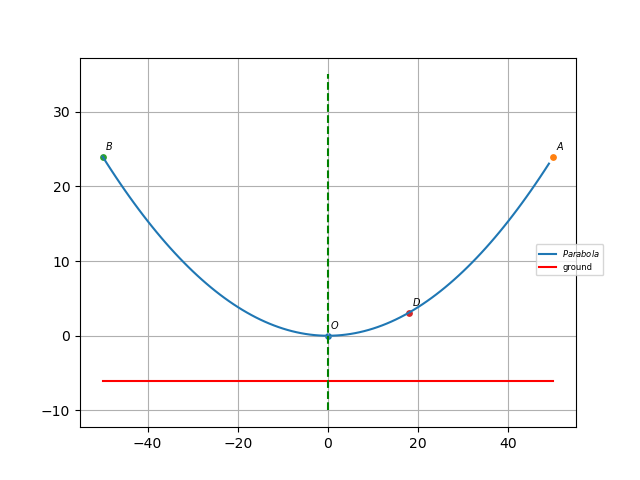
\includegraphics[width=0.75\columnwidth]{chapters/11/11/5/3/figs/parabola.png}
    \caption{}
    \label{fig:chapters/11/11/5/3/parabola}
\end{figure}


    \item Find the area of the triangle formed by the lines joining the vertex 
    of the parabola 
    \begin{align}
        x^2 = 12y
        \label{eq:chapters/11/11/5/6/parabola}
    \end{align}
    to the ends of its latus rectum.
\label{chapters/11/11/5/6}
%		Rewriting \eqref{eq:chapters/11/11/5/6/parabola} in matrix form,
    \begin{align}
        \vec{x}^\top\myvec{1&0\\0&0}\vec{x} + 2\myvec{0&-6}\vec{x} = 0
        \label{eq:chapters/11/11/5/6/parabola-mtx}
    \end{align}
    The above parabola can be  expressed in standard form using 
\begin{align}
	\vec{x} = \vec{P}\vec{y} = \myvec{0 & 1 \\ 1 & 0}\vec{y}
        \label{eq:chapters/11/11/5/6/affine}
\end{align}
yielding
    \begin{align}
        \vec{y}^\top\myvec{0&0\\0&1}\vec{x} + 2\myvec{-6&0}\vec{x} = 0
        \label{eq:chapters/11/11/5/6/parabola-mty}
    \end{align}
    Hence, 
    from
\eqref{eq:conic_quad_form_nc}, 
    \begin{align}
	    \vec{n} = \vec{e}_1
        \label{eq:chapters/11/11/5/6/n}
	\\
	    c = -\frac{36}{2\times 6} = -3
    \end{align}
    Substituting in 
  \eqref{eq:conic_quad_form_F} 
  yields
    \begin{align}
        \vec{F} = 3\vec{e}_1
    \end{align}
    Thus, the equation of the latus rectum is
\begin{align}
        \vec{x} = \vec{F} + \kappa \vec{e}_2
        \label{eq:chapters/11/11/5/6/x-general}
    \end{align}
        Substituting in \eqref{eq:chapters/11/11/5/6/parabola-mty} and simplifying,
    \begin{align}
\kappa = \pm 6
        \label{eq:chapters/11/11/5/6/x-latus}
    \end{align}
    Thus, the ends of the latus rectum are
    \begin{align}
        \vec{y} = \myvec{3 \\ \pm 6}
    \end{align}
    The relevant parameters with respect to 
        \eqref{eq:chapters/11/11/5/6/parabola-mtx}
	can now be obtained using 
        \eqref{eq:chapters/11/11/5/6/affine}.
See \figref{fig:chapters/11/11/5/6/parabola}.
The area of the required triangle is
    \begin{align}
        \textrm{ar}\brak{\triangle OAB} = \frac{1}{2}\mydet{6&3\\-6&3} = 18 
    \end{align}
    \begin{figure}[H]
        \centering
        %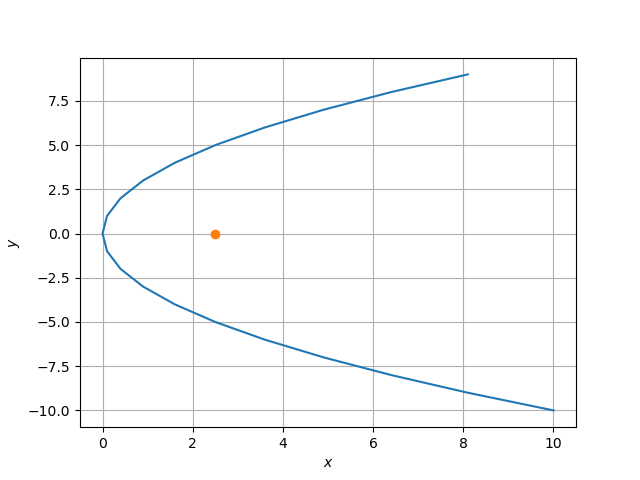
\includegraphics[width=0.75\columnwidth]{chapters/11/11/5/6/figs/parabola.png}
        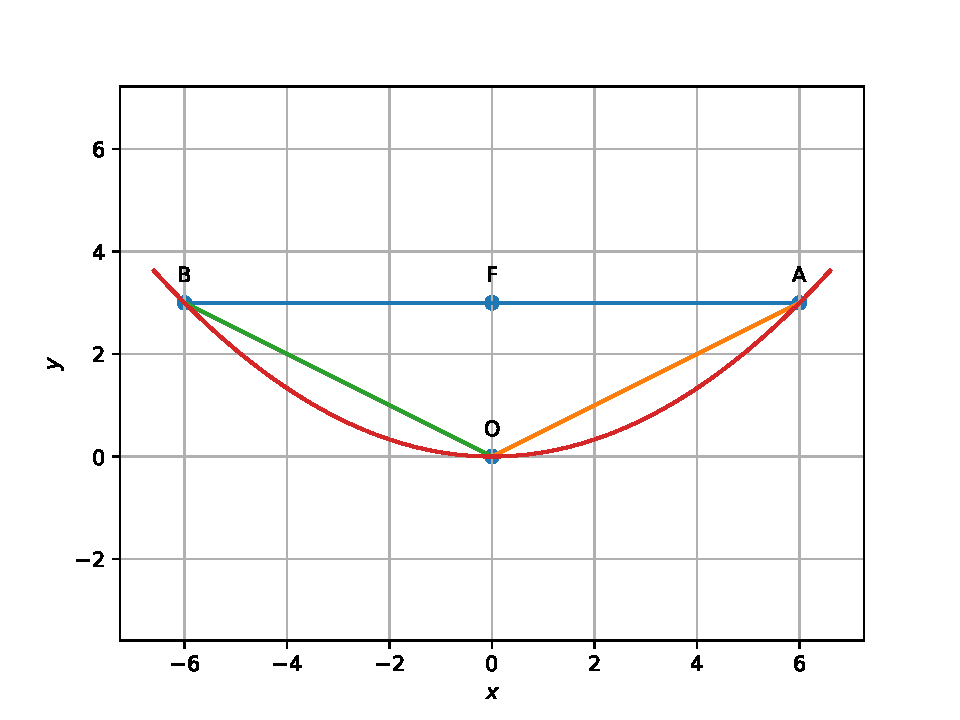
\includegraphics[width=0.75\columnwidth]{chapters/11/11/5/6/figs/fig1.pdf}
        \caption{}
        \label{fig:chapters/11/11/5/6/parabola}
    \end{figure}

\item An equilateral triangle is inscribed in the parabola $y^{2} = 4ax$,where one vertex is at the vertex of the parabola. Find the length of the side of the triangle.
\label{chapters/11/11/5/8}
%\iffalse
\documentclass[journal,10pt,twocolumn]{article}
\usepackage{graphicx}
\usepackage[margin=0.5in]{geometry}
\usepackage[cmex10]{amsmath}
\usepackage{array}
\usepackage{booktabs}
\usepackage{mathtools}
\usepackage{amssymb}
\title{\textbf{Conics Assignment}}
\author{Alavala Chinnapa Reddy}
\date{September 2022}
\providecommand{\norm}[1]{\left\lVert#1\right\rVert}
\providecommand{\abs}[1]{\left\vert#1\right\vert}
\let\vec\mathbf
\newcommand{\myvec}[1]{\ensuremath{\begin{pmatrix}#1\end{pmatrix}}}
\newcommand{\mydet}[1]{\ensuremath{\begin{vmatrix}#1\end{vmatrix}}}
\providecommand{\brak}[1]{\ensuremath{\left(#1\right)}}
\providecommand{\lbrak}[1]{\ensuremath{\left(#1\right.}}
\providecommand{\rbrak}[1]{\ensuremath{\left.#1\right)}}
\providecommand{\sbrak}[1]{\ensuremath{{}\left[#1\right]}}
\begin{document}

\maketitle
\paragraph{\textit{Problem Statement} -
\fi
An equilateral triangle is inscribed in the parabola $y^{2} = 4ax$,where one vertex is at the vertex of the parabola. Find the length of the side of the triangle.
	\begin{figure}[!ht]
		\centering
 \includegraphics[width=\columnwidth]{chapters/11/11/5/8/figs/co.pdf}
		\caption{}
		\label{fig:11/11/5/8}
  	\end{figure}
\\
\solution
\iffalse
} \vspace{5mm}
\section*{\large Solution}


Given, the axis of parabola is horizotal.
\\ Given,one vertex of $\triangle$OAB is at vertex of parabola.

\begin{figure}[h]
\includegraphics[width=0.8\columnwidth]{figs/co.pdf}
\end{figure}
\begin{equation}
  \label{eq:std_parabola}
  \textbf{x}^T\textbf{V}\textbf{x}+2\textbf{u}^T\textbf{x}+f=0
\end{equation}
where,
\begin{eqnarray}
	\vec{O}=\myvec{0\\0}
\end{eqnarray}	
Equation Parabola is $y^2=4ax$\\
From $\triangle$OAB
\begin{eqnarray}
	\norm{\vec{A}}=\norm{\vec{B}}=\norm{\vec{A-B}}\\
	\norm{\vec{A}}^2=\norm{\vec{B}}^2=\norm{\vec{A-B}}^2\\
	\norm{\vec{A}}^2+\norm{\vec{B}}^2-2\vec{A}^T\vec{B}=\norm{\vec{A}}^2=\norm{\vec{B}}^2\\
	\frac{\vec{A}^T\vec{B}}{\norm{\vec{A}}^2}=\frac{\vec{A}^T\vec{B}}{\norm{\vec{B}^2}}=\frac{1}{2}
\end{eqnarray}
$\triangle$OAB is a equilateral triangle\\
$\alpha$=$60^{0}$\\
The side length of equilateral triangle,OA=OB=AB=r\\
Let
\begin{eqnarray}
	\vec{A}=\myvec{r\cos{\theta_1}\\r\sin{\theta_1}}\\
	\vec{B}=\myvec{r\cos{\theta_2}\\r\sin{\theta_2}}
\end{eqnarray}
\begin{eqnarray}
	\vec{A}^T\vec{B}=\frac{\norm{\vec{A}}^2}{2}\\
	r^2\cos{(\theta_1-\theta_2)}=\frac{r^2}{2}\\
	\theta_1-\theta_2=\cos{^{-1}\frac{1}{2}}
\end{eqnarray}
Given $\vec{A}$ satisfy the eq1
\begin{eqnarray}
	\vec{A}^T\vec{V}\vec{A}+2\vec{u}^T\vec{A}+f=0\\
	\vec{A}^T\vec{V}\vec{A}+2\vec{u}^T\vec{A}=0
\end{eqnarray}
\begin{equation}
	\myvec{r\cos{\theta_1}&r\sin{\theta_1}}\myvec{0&0\\0&1}\myvec{r\cos{\theta_1}\\r\sin{\theta_1}}+2\myvec{-2a&0}\myvec{r\cos{\theta_1}\\r\sin{\theta_1}}=0
\end{equation}
\begin{equation}
	\myvec{r\cos{\theta_1}&r\sin{\theta_1}}\myvec{0\\r\sin{\theta_1}}+2(-2ar\cos{\theta_1})=0
\end{equation}
\begin{eqnarray}
	r^2\sin{^2\theta_1}=4ar\cos{\theta_1}\\
	r=\frac{4a\cos{\theta_1}}{\sin{^2\theta_1}}
\end{eqnarray}
Similarly $\vec{B}$ satisfy the eq1
\begin{equation}
	r=\frac{4a\cos{\theta_2}}{\sin{^2\theta_2}}
\end{equation}
Form eq17 and eq18\\
Yeilding
\begin{eqnarray}
	\cos{(\theta_1+\theta_2)}=1\\
	\theta_1+\theta_2=\cos{^{-1}1}
\end{eqnarray}
Add eq11 and eq20\\
\begin{equation}
	\theta_1=\frac{\cos{^{-1}\frac{1}{2}+\cos{^{-1}1}}}{2}
\end{equation}
Subtract eq20 from eq11
\begin{equation}   
\theta_2=\frac{-\cos{^{-1}\frac{1}{2}+\cos{^{-1}1}}}{2}        
\end{equation}
 \section*{\large Construction} The input parameters are V,u,f \\
 $\vec{V}=\myvec{0&0\\0&1},\vec{u}=\myvec{-2a\\0},f=0$\\
\setlength\extrarowheight{7pt}
\begin{tabular}{|c|c|c|}
  \hline
  \textbf{Symbol}&\textbf{Value}&\textbf{Description}\\
  \hline
	a&1&\\
  \hline
	$\alpha$&$60^{0}$&$\angle{A}=\angle{B}=\angle{O}$\\
	\hline
	r&Solving eq18&OA=OB=AB\\
	\hline
  $\vec{O}$&$\myvec{0\\0}$&center of parabola and Point O\\
  \hline
	$\vec{A}$&$\myvec{r\cos{\theta_1}\\r\sin{\theta_1}}$&Point A\\[8pt]
  \hline
	$\vec{B}$&$\myvec{r\cos{\theta_2}\\r\sin{\theta_2}}$&Point B\\[8pt]  \hline
\end{tabular}
\end{document}
\fi

\item An arch is in the form of a semi-ellipse. It is 8 m wide and 2 m high at the centre. Find the height of the arch at a point 1.5 m from one end.
\label{chapters/11/11/5/4}
%\iffalse
\def\mytitle{PYTHON PROGRAMMING ON MATRICES}
\def\myauthor{K.Pavan Kumar}
\def\contact{r170850@rguktrkv.ac.in}
\def\mymodule{Future Wireless Communication (FWC)}
\documentclass[10pt, a4paper]{article}
\usepackage[a4paper,outer=1.5cm,inner=1.5cm,top=1.75cm,bottom=1.5cm]{geometry}
\twocolumn
\usepackage{graphicx}
\graphicspath{{./images/}}
\usepackage[colorlinks,linkcolor={black},citecolor={blue!80!black},urlcolor={blue!80!black}]{hyperref}
\usepackage[parfill]{parskip}
\usepackage{lmodern}
\usepackage{tikz}
	\usepackage{physics}
\usepackage{tabularx}
\usepackage{enumitem}
\usetikzlibrary{calc}
\usepackage{amsmath}
\usepackage{amssymb}
\renewcommand*\familydefault{\sfdefault}
\usepackage{watermark}
\usepackage{lipsum}
\usepackage{xcolor}
\usepackage{listings}
\usepackage{float}
\usepackage{titlesec}
\providecommand{\mtx}[1]{\mathbf{#1}}
\titlespacing{\subsection}{1pt}{\parskip}{3pt}
\titlespacing{\subsubsection}{0pt}{\parskip}{-\parskip}
\titlespacing{\paragraph}{0pt}{\parskip}{\parskip}


\newcommand{\myvec}[1]{\ensuremath{\begin{pmatrix}#1\end{pmatrix}}}
\let\vec\mathbf
\lstset{
frame=single, 
breaklines=true,
columns=fullflexible
}
\thiswatermark{\centering \put(0,-110.0){
\includegraphics[scale=0.3]{logo.png}} }
\title{\mytitle}
\author{\myauthor\hspace{1em}\\\contact\\FWC22011\hspace{6.5em}IITH\hspace{0.5em}\mymodule\hspace{6em}Matrix:conic}
\date{}
\begin{document}
	\maketitle
	\tableofcontents
   \section{Problem}
   \fi
\\
\solution 
	\begin{figure}[!ht]
		\centering
 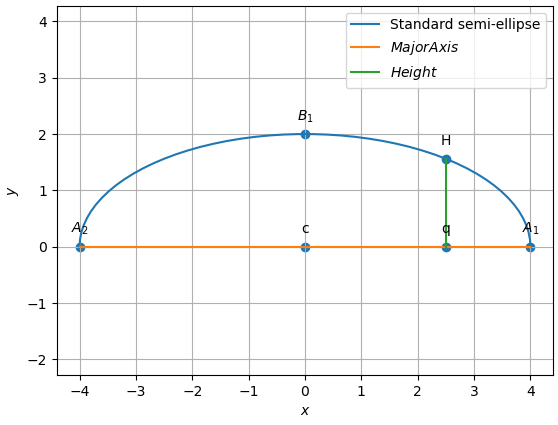
\includegraphics[width=\columnwidth]{chapters/11/11/5/4/figs/ellipse.png}
		\caption{}
		\label{fig:11/11/5/4}
  	\end{figure}
	\iffalse

\section{Construction}
  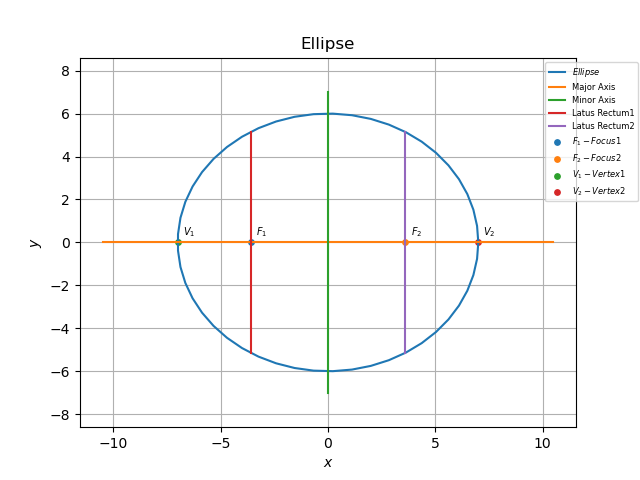
\includegraphics[scale=0.45]{ellipse.png}
  	\begin{center}
  Figure of construction
  	\end{center}
  \section{Solution}
Ellipse equation:
\begin{align}
\frac{x^2}{16}+\frac{y^2}{4}=1
\end{align}
The standard equation of the conics is given as :
\begin{align}
\vec{x}^{\top}\vec{V}\vec{x}+2\vec{u}^{\top}\vec{x}+f=0
\label{eq:conic}
\end{align}

The given ellipse can be expressed in  conics as\\ 
\begin{align}
\vec{u} = \myvec{0 \\0} , f =-1 
\end{align}


    The input parameters for this construction are
\begin{center}
\begin{tabular}{|c|c|c|}
	\hline
	\textbf{Symbol}&\textbf{Value}&\textbf{Description}\\
	\hline
	$a$ &4&Length of semi major axis\\
	\hline
    $b$ &2&Length of semi minor axis\\
    \hline
    $\vec{e_1}$ &\myvec{1\\0}&Standard basis vector along X-axis \\
	\hline
    $\vec{m}$ & $\myvec{0\\1}$ &Directional vector along Y-axis\\
	\hline
\end{tabular}


    The steps for constructing above figure are :
\begin{enumerate}
 \item Generate semi-ellipse with semi major axis and semi minor axis lengths equal to $\vec{a}$ and $\vec{b}$ respectively.
 \item Locate center $\vec{c}$ and vertices $\vec{A_1}$ and $\vec{A_2}$.
 \item Locate point $\vec{q}$ on the major axis.
 \item Find the height of ellipse at $\vec{q}$ .
\end{enumerate}

For the standard ellipse, the length of the major axis and minor axis are:
\begin{align}
2\sqrt{\abs{\frac{f_0}{\lambda_1}}} \\
2\sqrt{\abs{\frac{f_0}{\lambda_2}}} 
\end{align}

Given ,The major axis and minor axis are 8m and 4m in length respectively. \\
$*f_0=\vec{u}^{\top} \vec{v}^{-1}\vec{u}-f=1$ 


Equation (5)$\implies2\sqrt{\abs{\frac{f_0}{\lambda_1}}}$=8\\
$\implies\lambda_1$=1/16

Equation (6)$\implies2\sqrt{\abs{\frac{f_0}{\lambda_2}}}$=4\\
$\implies\lambda_2$=1/4

\begin{align}
   \implies \vec{v}=\myvec{\lambda_1&0\\0&\lambda_2}=\myvec{1/16&0\\0&1/4}
\end{align}


\textbf{vertices:}            $\vec{v}=\pm a\vec{e_1}$
\begin{align}
\vec{v}=\pm a\myvec{1\\0} =\pm\myvec{4\\0}\\
Let, \vec{A_1}=\myvec{4 \\0},\vec{A_2}=\myvec{-4 \\0}
\end{align}


 To find the height of ellipse at a point 1.5m from end,
 \begin{align}
\implies\norm{\vec{A_1}-\vec{q}}^2 = (1.5)^2 \\
(\vec{A_1}-\vec{q})^\top(\vec{A_1}-\vec{q})=(1.5)^2\\
\norm{\vec{A_1}^2}+\norm{\vec{q}^2}-2\vec{A_1}^{\top}\vec{q}=(1.5)^2\\
\norm{\vec{q}}^2-2\vec{A}^\top\vec{q}+13.75=0\\
 \vec{e_2}^\top\vec{q}=0 \\
 \implies \vec{q}=\lambda\vec{e_1} 
\end{align}
substitute (14) in (12);
$\implies \lambda^2-8\lambda+13.75=0$\\
$\implies\lambda=\frac{5}{2},\frac{11}{2}$\\
The length of semi major axis is 4m,we need to find height of ellipse at a point 1.5m from one end.
\\$\therefore$ the possible solution  is $\lambda=\frac{5}{2}$
\\$\lambda$ lies on x-axis.
 \begin{align} 
\implies \vec{q}=\myvec{\frac{5}{2}\\0}
\end{align}



\textbf{Directional vector m:}\\
The unit vector along $\vec{Y}$-axis become the directional vector along $\vec{Y}$-axis.
\begin{align}
    \implies\vec{m}=\myvec{0\\1}
\end{align}

\end{center}
\textbf{Theorem:}
The points of intersection of the line 
\begin{align}
L: \quad \vec{x} = \vec{q} + \mu \vec{m} \quad \mu \in \mathbb{R}
\end{align}
with the conic section in \eqref{eq:conic} are given by
\begin{align}
\vec{x}_i = \vec{q} + \mu_i \vec{m}
\end{align}

where $\mu_i$ is given by  \\
\begin{align}
\mu_i =\frac{1}
{\vec{m}^{\top}\vec{V}\vec{m}}
\left(-\vec{m}^{\top}(\vec{V}\vec{q}+\vec{u}) \pm Z\right) 
\end{align}
\\
\\
 Z = $\sqrt{[\vec{m}^{\top}(\vec{V}\vec{q}+\vec{u})]^2 -(\vec{q}^{\top}\vec{V}\vec{q} + 2\vec{u}^{\top}\vec{q} +f)(\vec{m}^{\top}\vec{V}\vec{m})}$
 \\
 \\

By substituting the vectors $\vec{m}$,$\vec{q}$,$\vec{v}$,$\vec{u}$ and constant f in  (19) results intersection points on the conic section .Consider absolute value ,say $\vec{H}$.

 $\vec{H}$ gives height of ellipse at point $\vec{q}$.

\begin{center}
    (or)
\end{center}
        
 $\norm{\vec{H}-\vec{q}}$ results the same.\\
  $\therefore$ Height of ellipse at $\vec{q}$=1.56.

\textbf{termux commands :}
\begin{lstlisting}
bash conic.sh............using shell command
\end{lstlisting}

\begin{center}
Below python code realizes the above construction :
\fbox{\parbox{8.5cm}{\url{https://github.com/FWC_module1/blob/main/matrices/conic/conic.py}}}
\end{center}
\end{document}
\fi

\item A rod of length 12cm moves with its ends always touching the coordinate axes. Determine the equation of locus of a point  P on the rod, which is 3cm from the end in contact with $x-axis$.
\label{chapters/11/11/5/5}
%\iffalse
\documentclass[journal,11pt,twocolumn]{IEEEtran}
%
\usepackage{setspace}
\usepackage{gensymb}
%\doublespacing
\singlespacing

%\usepackage{graphicx}
%\usepackage{amssymb}
%\usepackage{relsize}
\usepackage[cmex10]{amsmath}
%\usepackage{amsthm}
%\interdisplaylinepenalty=2500
%\savesymbol{iint}
%\usepackage{txfonts}
%\restoresymbol{TXF}{iint}
%\usepackage{wasysym}
\usepackage{amsthm}
%\usepackage{iithtlc}
\usepackage{mathrsfs}
\usepackage{txfonts}
\usepackage{stfloats}
\usepackage{bm}
\usepackage{cite}
\usepackage{cases}
\usepackage{subfig}
%\usepackage{xtab}
\usepackage{longtable}
\usepackage{multirow}
%\usepackage{algorithm}
%\usepackage{algpseudocode}
\usepackage{enumitem}
\usepackage{mathtools}
\usepackage{steinmetz}
\usepackage{tikz}
\usepackage{circuitikz}
\usepackage{verbatim}
\usepackage{tfrupee}
\usepackage[breaklinks=true]{hyperref}
%\usepackage{stmaryrd}
\usepackage{tkz-euclide} % loads  TikZ and tkz-base
%\usetkzobj{all}
\usetikzlibrary{calc,math}
\usepackage{listings}
    \usepackage{color}                                            %%
    \usepackage{array}                                            %%
    \usepackage{longtable}                                        %%
    \usepackage{calc}                                             %%
    \usepackage{multirow}                                         %%
    \usepackage{hhline}                                           %%
    \usepackage{ifthen}                                           %%
  %optionally (for landscape tables embedded in another document): %%
    \usepackage{lscape}     
\usepackage{multicol}
\usepackage{chngcntr}
%\usepackage{enumerate}

%\usepackage{wasysym}
%\newcounter{MYtempeqncnt}
\DeclareMathOperator*{\Res}{Res}
%\renewcommand{\baselinestretch}{2}
\renewcommand\thesection{\arabic{section}}
\renewcommand\thesubsection{\thesection.\arabic{subsection}}
\renewcommand\thesubsubsection{\thesubsection.\arabic{subsubsection}}

\renewcommand\thesectiondis{\arabic{section}}
\renewcommand\thesubsectiondis{\thesectiondis.\arabic{subsection}}
\renewcommand\thesubsubsectiondis{\thesubsectiondis.\arabic{subsubsection}}

% correct bad hyphenation here
\hyphenation{op-tical net-works semi-conduc-tor}
\def\inputGnumericTable{}                                 %%

\lstset{
%language=C,
frame=single, 
breaklines=true,
columns=fullflexible
}
%\lstset{
%language=tex,
%frame=single, 
%breaklines=true
%}

\begin{document}
%


\newtheorem{theorem}{Theorem}[section]
\newtheorem{problem}{Problem}
\newtheorem{proposition}{Proposition}[section]
\newtheorem{lemma}{Lemma}[section]
\newtheorem{corollary}[theorem]{Corollary}
\newtheorem{example}{Example}[section]
\newtheorem{definition}[problem]{Definition}
%\newtheorem{thm}{Theorem}[section] 
%\newtheorem{defn}[thm]{Definition}
%\newtheorem{algorithm}{Algorithm}[section]
%\newtheorem{cor}{Corollary}
\newcommand{\BEQA}{\begin{eqnarray}}
\newcommand{\EEQA}{\end{eqnarray}}
\newcommand{\define}{\stackrel{\triangle}{=}}

\bibliographystyle{IEEEtran}
%\bibliographystyle{ieeetr}


\providecommand{\mbf}{\mathbf}
\providecommand{\pr}[1]{\ensuremath{\Pr\left(#1\right)}}
\providecommand{\qfunc}[1]{\ensuremath{Q\left(#1\right)}}
\providecommand{\sbrak}[1]{\ensuremath{{}\left[#1\right]}}
\providecommand{\lsbrak}[1]{\ensuremath{{}\left[#1\right.}}
\providecommand{\rsbrak}[1]{\ensuremath{{}\left.#1\right]}}
\providecommand{\brak}[1]{\ensuremath{\left(#1\right)}}
\providecommand{\lbrak}[1]{\ensuremath{\left(#1\right.}}
\providecommand{\rbrak}[1]{\ensuremath{\left.#1\right)}}
\providecommand{\cbrak}[1]{\ensuremath{\left\{#1\right\}}}
\providecommand{\lcbrak}[1]{\ensuremath{\left\{#1\right.}}
\providecommand{\rcbrak}[1]{\ensuremath{\left.#1\right\}}}
\theoremstyle{remark}
\newtheorem{rem}{Remark}
\newcommand{\sgn}{\mathop{\mathrm{sgn}}}
\providecommand{\abs}[1]{\left\vert#1\right\vert}
\providecommand{\res}[1]{\Res\displaylimits_{#1}} 
\providecommand{\norm}[1]{\left\lVert#1\right\rVert}
%\providecommand{\norm}[1]{\lVert#1\rVert}
\providecommand{\mtx}[1]{\mathbf{#1}}
\providecommand{\mean}[1]{E\left[ #1 \right]}
\providecommand{\fourier}{\overset{\mathcal{F}}{ \rightleftharpoons}}
%\providecommand{\hilbert}{\overset{\mathcal{H}}{ \rightleftharpoons}}
\providecommand{\system}{\overset{\mathcal{H}}{ \longleftrightarrow}}
	%\newcommand{\solution}[2]{\textbf{Solution:}{#1}}
\newcommand{\solution}{\noindent \textbf{Solution: }}
\newcommand{\cosec}{\,\text{cosec}\,}
\providecommand{\dec}[2]{\ensuremath{\overset{#1}{\underset{#2}{\gtrless}}}}
\newcommand{\myvec}[1]{\ensuremath{\begin{pmatrix}#1\end{pmatrix}}}
\newcommand{\mydet}[1]{\ensuremath{\begin{vmatrix}#1\end{vmatrix}}}
%\numberwithin{equation}{section}
\numberwithin{equation}{subsection}
%\numberwithin{problem}{section}
%\numberwithin{definition}{section}
\makeatletter
\@addtoreset{figure}{problem}
\makeatother

\let\StandardTheFigure\thefigure
\let\vec\mathbf
%\renewcommand{\thefigure}{\theproblem.\arabic{figure}}
\renewcommand{\thefigure}{\theproblem}
%\setlist[enumerate,1]{before=\renewcommand\theequation{\theenumi.\arabic{equation}}
%\counterwithin{equation}{enumi}


%\renewcommand{\theequation}{\arabic{subsection}.\arabic{equation}}

\def\putbox#1#2#3{\makebox[0in][l]{\makebox[#1][l]{}\raisebox{\baselineskip}[0in][0in]{\raisebox{#2}[0in][0in]{#3}}}}
     \def\rightbox#1{\makebox[0in][r]{#1}}
     \def\centbox#1{\makebox[0in]{#1}}
     \def\topbox#1{\raisebox{-\baselineskip}[0in][0in]{#1}}
     \def\midbox#1{\raisebox{-0.5\baselineskip}[0in][0in]{#1}}

\vspace{3cm}


\title{Que: 11.11.5.5}
\author{Nikam Pratik Balasaheb (EE21BTECH11037)}





% make the title area
\maketitle

\newpage

%\tableofcontents

\bigskip

\renewcommand{\thefigure}{\theenumi}
\renewcommand{\thetable}{\theenumi}
%\renewcommand{\theequation}{\theenumi}

\section{Problem}


\section{Solution}
\fi
Let the angle made by the rod with x-axis be $\theta$.  Then
\begin{enumerate}

\item x-intercept:
	\begin{align}
	\vec{A} = \myvec{12\cos{\theta}\\0}
	\end{align}

\item y-intercept:
	\begin{align}
		\vec{B} =\myvec{0\\12\sin{\theta}}
	\end{align}

\item direction vector of rod:
	\begin{align}
		\vec{A}-\vec{B} = 12\myvec{\cos{\theta} \\ -\sin{\theta}}
	\end{align}
	Unit vector along direction vector:
	\begin{align}
		\vec{m} = \myvec{\cos{\theta} \\ -\sin{\theta}}
	\end{align}

\item given point $\vec{P}$:
	\begin{align}
		\vec{P} &= \vec{A} - 3 \vec{m}\\
			&= \myvec{9 \cos{\theta} \\ 3 \sin{\theta}}
	\end{align}
\item parametric form of locus:
	\begin{align}
		\vec{x} = \myvec{9\cos{\theta} \\ 3\sin{\theta}}\\
	\end{align}
	Consider $\vec{Q} = \myvec{\frac{1}{9}&0\\0&\frac{1}{3}}$
	\begin{align}
		\vec{Q}\vec{x} &= \myvec{\cos{\theta}\\ \sin{\theta}}\\
		\norm{\vec{Q}\vec{x}}^2 &= 1\\
		\brak{\vec{Q}\vec{x}}^{\top} \brak{\vec{Q}\vec{x}} &= 1\\
		\vec{x}^{\top}\vec{Q}^{\top}\vec{Q}\vec{x} &= 1\\
		\vec{x}^T\myvec{\frac{1}{81} & 0 \\ 0 & \frac{1}{9}} \vec{x} &= 1
	\end{align}
	The locus of point $\vec{P}$ is a conic 
	\begin{align}\vec{x}^{\top} \vec{V} \vec{x} + 2 \vec{u}^{\top} \vec{x} +f= 0
	\end{align}
	where,
	\begin{align}
		\vec{V} &= \myvec{\frac{1}{81}&0\\0&\frac{1}{9}}\\
		\vec{u} &= \myvec{0\\0}\\
		f &= -1
	\end{align}
\end{enumerate}
See Table 
	\ref{tab:chapters/11/11/5/5/}.
\begin{table}[h!]
	\begin{center}
		%%%%%%%%%%%%%%%%%%%%%%%%%%%%%%%%%%%%%%%%%%%%%%%%%%%%%%%%%%%%%%%%%%%%%%
%%                                                                  %%
%%  This is a LaTeX2e table fragment exported from Gnumeric.        %%
%%                                                                  %%
%%%%%%%%%%%%%%%%%%%%%%%%%%%%%%%%%%%%%%%%%%%%%%%%%%%%%%%%%%%%%%%%%%%%%%

\begin{tabular}[]{|c|c|c|}
\hline
Parameter	& Value	& Description \\ \hline
$\vec{A}$	& $\myvec{12 \cos{\theta}\\0}$ & x-intercept of rod \\ \hline
$\vec{C}$	& $\myvec{0\\ 12 \sin{\theta}}$ & y-intercept of the rod\\ \hline
$\vec{P}$	& $\myvec{9 \cos{\theta} \\ 3\sin{\theta}}  $ & Point on rod, at given distance from $\vec{A} $ \\ \hline
$\theta$ 		& $\frac{\pi}{3}$ & parameter $\theta$ for $\vec{A}, \vec{B},\vec{P}$\\[1pt] \hline
length	& 12 	& Length of the rod \\ \hline
dist	& 3	& Distance between $\vec{A}, \vec{P}$\\ \hline
\end{tabular}

	\end{center}
	\caption{}
	\label{tab:chapters/11/11/5/5/}
\end{table}
See Fig.
    \ref{fig:chapters/11/11/5/5/}
\begin{figure}[h!]
  \centering
    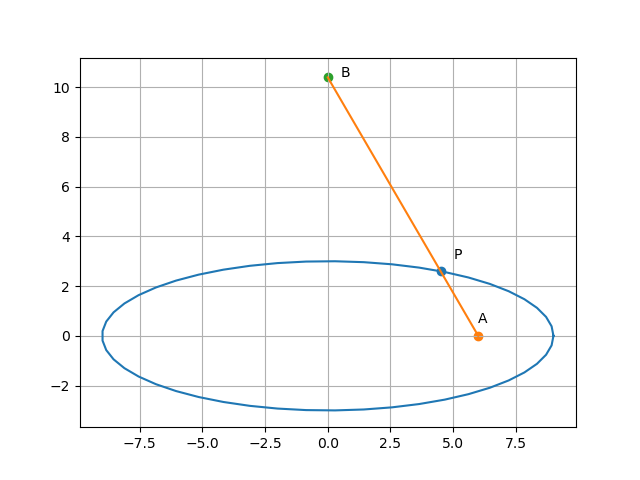
\includegraphics[width=\columnwidth]{chapters/11/11/5/5/figs/Figure_1.png}
    \caption{}
    \label{fig:chapters/11/11/5/5/}
\end{figure}





\item A man running a racecourse notes that the sum of the distances from the two flag posts from him is always 10 m and the distance between the flag posts is 8 m. Find the equation of the posts traced by the man. 
\label{chapters/11/11/5/7}
%\iffalse
\documentclass[12pt]{article}
\usepackage{graphicx}
\usepackage[none]{hyphenat}
\usepackage{graphicx}
\usepackage{listings}
\usepackage[english]{babel}
\usepackage{graphicx}
\usepackage{caption} 
\usepackage{booktabs}
\usepackage{array}
\usepackage{amssymb} % for \because
\usepackage{amsmath}   % for having text in math mode
\usepackage{extarrows} % for Row operations arrows
\usepackage{listings}
\lstset{
  frame=single,
  breaklines=true
}
\usepackage{hyperref}
  
%Following 2 lines were added to remove the blank page at the beginning
\usepackage{atbegshi}% http://ctan.org/pkg/atbegshi
\AtBeginDocument{\AtBeginShipoutNext{\AtBeginShipoutDiscard}}


%New macro definitions
\newcommand{\mydet}[1]{\ensuremath{\begin{vmatrix}#1\end{vmatrix}}}
\providecommand{\brak}[1]{\ensuremath{\left(#1\right)}}
\providecommand{\norm}[1]{\left\lVert#1\right\rVert}
\providecommand{\abs}[1]{\left\vert#1\right\vert}
\newcommand{\solution}{\noindent \textbf{Solution: }}
\newcommand{\myvec}[1]{\ensuremath{\begin{pmatrix}#1\end{pmatrix}}}
\let\vec\mathbf


\begin{document}

\begin{center}
\title{\textbf{Conic Sections - Ellipse}}
\date{\vspace{-5ex}} %Not to print date automatically
\maketitle
\end{center}
\setcounter{page}{1}

\section{11$^{th}$ Maths - Chapter 11}
This is Problem-7 from Exercise 11.5
\begin{enumerate}

\solution 
\fi
The conic section for the given problem is an ellipse. Let $\vec{O}\myvec{0 \\ 0}$ be the centre of the Ellipse. Then, the focii are given by 
\begin{align}
    \label{eq:chapters/11/11/5/7/ellipseEq1}
	\vec{F_1} = \myvec{ 4 \\ 0} \\
	\vec{F_2} = \myvec{ -4 \\ 0} 
\end{align}
The sum of the distances from two focii to the point on the locus of the ellipse is equal to $10m$. Let $\vec{P}\myvec{p \\ 0 }$ and $\vec{Q}\myvec{-q \\ 0}$ be the vertices of the ellipse. Then
\begin{align}
	\norm{\vec{P}-\vec{F_1}} + \norm{\vec{P}-\vec{F_2}} = 10 \\
         \brak{p-4} + \brak{p+4} = 10 \\
	 2p = 10 \\
	 p = 5  \\
	 \therefore \vec{P} = \myvec{5 \\ 0}
\end{align}
Similarly
\begin{align}
	\norm{\vec{Q}-\vec{F_1}} + \norm{\vec{Q}-\vec{F_2}} = 10 \\
         \brak{q-4} + \brak{q+4} = 10 \\
	 2q = 10 \\
	 q = 5 \\
	 \therefore \vec{Q} = \myvec{-5 \\ 0}
\end{align}
We know that the Vertex of a standard ellipse is given by
\begin{align}
	\vec{P} &=  \myvec{\sqrt{\abs{\frac{f_0}{\lambda_1}}} \\ 0} \\
	\myvec{5 \\ 0} &=  \myvec{\sqrt{\abs{\frac{f_0}{\lambda_1}}} \\ 0} \\
	\frac{f_0}{\lambda_1} &= 25 \\
	\label{eq:chapters/11/11/5/7/eqV}
	f_0 &= 25\lambda_1 
\end{align}
We know that the Focii for standard Ellipse are given as
\begin{align}
	\label{eq:chapters/11/11/5/7/eqV1}
	\vec{F} &= \pm e\sqrt{\frac{\abs{f_0}}{\lambda_2\brak{1-e^2}}}\vec{e}_1
\end{align}
Substituting values of $\vec{F_1}$ from \eqref{eq:chapters/11/11/5/7/ellipseEq1} and $f_0$ from \eqref{eq:chapters/11/11/5/7/eqV}
\begin{align}
	   \label{eq:chapters/11/11/5/7/eqV2}
	   \eqref{eq:chapters/11/11/5/7/eqV1} \implies \myvec{4 \\0}  &=e\sqrt{\frac{25\lambda_1}{\lambda_2\brak{1-e^2}}}\vec{e}_1
\end{align}
We know that 
\begin{align}
	1-e^2 = \frac{\lambda_1}{\lambda_2} \\
	\eqref{eq:chapters/11/11/5/7/eqV2} \implies  4 &= 5e \\
        e &= \frac{4}{5} \\
	\therefore \frac{\lambda_1}{\lambda_2} &= 1 - \brak{\frac{4}{5}}^2 \\
	&= \frac{9}{25} \\
	\vec{n} &= \sqrt{\frac{\lambda_2}{f_0}}\vec{e}_1\\
	 &= \sqrt{\frac{\lambda_2}{25\lambda_1}}\vec{e}_1\\
	 &= \frac{1}{5} \times \frac{5}{3}\vec{e}_1\\
	 &= \frac{1}{3}\vec{e}_1 \\
	 c &= \frac{1}{e\sqrt{1-e^2}} = \frac{25}{12}
\end{align}
For the standard ellipse, $f$ is given as 
\begin{align}
	\label{eq:chapters/11/11/5/7/eqV3}
	f &= \norm{\vec{n}}^2 \norm{\vec{F}}^2 - c^2 e^2 \\
	&= \brak{\frac{1}{3}}^216 - \frac{25}{9} \\
	&= -1 \\
	f_0 &= -f = 1 \\
	\lambda_1 &= \frac{f_0}{25} = \frac{1}{25}\\
	\lambda_2 &= \frac{25\lambda_1}{9} = \frac{1}{9} \\
	\therefore \vec{V} &= \myvec{\lambda_1 & 0 \\ 0 & \lambda_2} = \myvec{\frac{1}{25} & 0 \\ 0 & \frac{1}{9}}
\end{align}
For a standard ellipse, $\vec{u}=0$. 

The generic equation of conic section is given as
\begin{align}
	\label{eq:chapters/11/11/5/7/ellipseEq2}
	g\brak{\vec{x}} &= \vec{x}^T\vec{V}\vec{x} + 2\vec{u}^T\vec{x} + f = 0 \\ 
	&= \vec{x}^T\myvec{\frac{1}{25} & 0 \\ 0 & \frac{1}{9}}\vec{x}- 1  = 0 
\end{align}
The relevant diagram is shown in Figure \ref{fig:chapters/11/11/5/7/Fig1}
\begin{figure}[!h]
	\begin{center}
		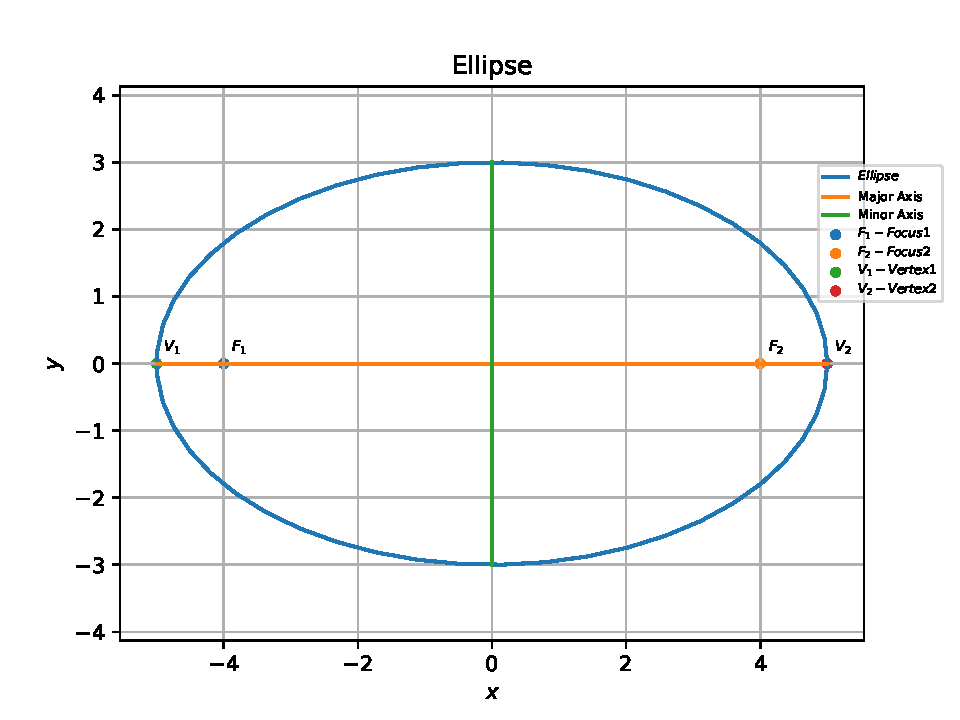
\includegraphics[width=\columnwidth]{chapters/11/11/5/7/figs/problem7.pdf}
	\end{center}
\caption{}
\label{fig:chapters/11/11/5/7/Fig1}
\end{figure}

\item The locus of the point of intersecton of lines $\sqrt{3}x+y-4\sqrt{3}k=0$ and $\sqrt{3}=0\sqrt{3}kx+ky-4\sqrt{3}=0$ for different value of K is a hyperboia whose eccentricity is 2.
\item lf $e$ is the eccentricity of the ellipes $\frac{x^2}{a^2}+\frac{y^2}{b^2}=1(a<b)$,then
\begin{enumerate}
\item $b^2=a^2(1-e^2)$
\item $a^2=b^2(1-e^2)$
\item $a^2=b^2(e^-1)$
\item $b^2=a^2(e^2-1)$
\end{enumerate}
\item An ellipse is described by using an endless string which is passed over two pins lf the oxes are 6cm and 4cm, the length of the string and distance between the pins are  \makebox[1cm]{\hrulefill}             
 \item Find the coordinates of a point on the parabola $y^2=8x$ whose focal distance is 4.
 \item Find the length of the line segment joining the vertex of the parabola $y^2=4ax$ and a point on the parabola where the line segment makes an angle 0 to the x-axis.
\item show that the set of all points such that the difference of their distances from (4,0) and (-4,0) is always equal to 2 represent a hyperbola .
\item If the distance between the foci of a hyperbola is 16 and its eccentricity is $\sqrt{2}$, then obtain the equation of the hyperbola.
\item The eccentricity of the hyperbola whose latus rectum is 8 and conjugate axis is equal to half of the distance between the foci is 
\begin{enumerate}
\item $4\pm3$
\item $\frac{4}{\sqrt{3}}$
\item $\frac{2}{\sqrt{3}}$
\item none of these
\end{enumerate}
\item The distance between the foci of a hyperbola is 16 and its eccentricity is $\le{2}$. lts equation is
\begin{enumerate}
\item $x^2-y^2=3^2$
\item $\frac{x^2}{4-}\frac{y^2}{9}=1$
\item $2x-3y^2=7$
 \item none of these
 \end{enumerate}
 \item If the latus rectum of an ellipse is equal to half of minor axis, then find its eccentricity.
 \item If the eccentricity of an ellipse is $\frac{5}{8}$ and  the distance between its foci is 10 then find latus rectum of the ellipse.
 \item Find the distance between the directrices of the ellipse $\frac{x^2}{36}+\frac{y^2}{20}$
\item Find the equation of the set of all points the sum of whose distances  from the points (3,0) and (9,0) is 12.
\item If ${P}$ is a point on the ellipse $\frac{x^2}{16}+\frac{y^2}{25}=1$ whose foci  are $s$ and $s'$ then $Ps +Ps'=8$.
\end{enumerate}
